\section{Method of Measuring Force}
To guide the robot using human force, the orthodox method is to first estimate the force applied on the robot then executes a behavior as described in figure \ref{fig:orthodox}.

\begin{figure}[!h]
\begin{center}
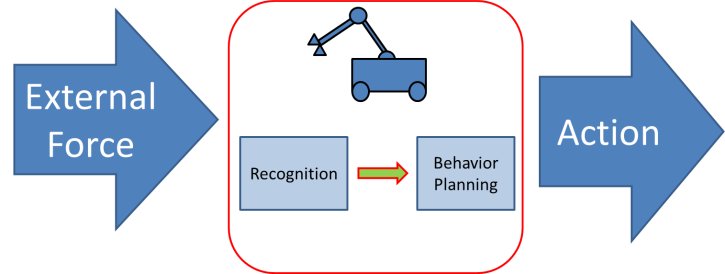
\includegraphics[width=9cm]{orthodox_method.png}
\caption{orthodox method}
\label{fig:orthodox}
\end{center}
\end{figure}

We attempted to estimate contact force on robotic manipulators in figure \ref{fig:manipulator}. There are two methods to measuring external force. 

\begin{enumerate}
\item Using force sensors to measure applied force.
\item Estimating applied force from joint torque. A common method is to use the current to find the torque as torque and current are proportional. Another method is using joint error positions to find the torque.
\end{enumerate}

\begin{figure}[!h]
\begin{center}
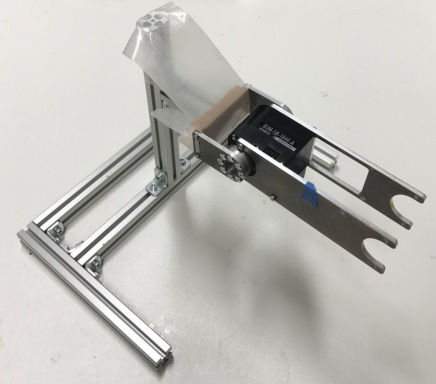
\includegraphics[width=5cm]{manipulator.jpg}
\caption{manipulator with a single DOF}
\label{fig:manipulator}
\end{center}
\end{figure}

Force sensors provide accurate measurement but cannot measure any force beyond their placement. On the other hand, estimating force from joint torque is difficult to obtain as estimation must also considered torque applied to hold the manipulator. 

There are limitations in using orthodox method. Measuring or estimating external force has a tradeoff between flexibility and accuracy. It is also difficult to write a rule for behavior selection for each joint state combination.
